%課題研究レジュメテンプレート ver. 1.2

\documentclass[uplatex]{jsarticle}
\usepackage[top=20mm,bottom=20mm,left=20mm,right=20mm]{geometry}
\usepackage[T1]{fontenc}
\usepackage{txfonts}
\usepackage{wrapfig}
\usepackage[expert,deluxe]{otf}
\usepackage[dvipdfmx,hiresbb]{graphicx}
\usepackage[dvipdfmx]{hyperref}
\usepackage{pxjahyper}
\usepackage{secdot}

\makeatletter
  \renewcommand{\section}{%
    \if@slide\clearpage\fi
    \@startsection{section}{1}{\z@}%
    {\Cvs \@plus.5\Cdp \@minus.2\Cdp}% 前アキ
    {.5\Cvs \@plus.3\Cdp}% 後アキ
    %{\normalfont\Large\headfont\raggedright}}
    {\normalfont\raggedright}}

  \renewcommand{\subsection}{\@startsection{subsection}{2}{\z@}%
    {\Cvs \@plus.5\Cdp \@minus.2\Cdp}% 前アキ
    {.5\Cvs \@plus.3\Cdp}% 後アキ
    %{\normalfont\large\headfont}}
    {\normalfont}}

  \renewcommand{\subsubsection}{\@startsection{subsubsection}{3}{\z@}%
    {\Cvs \@plus.5\Cdp \@minus.2\Cdp}%
    {\z@}%
    %{\normalfont\normalsize\headfont}}
    {\normalfont}}
\makeatother
%ここから上を編集する必要はない.






\title{\vspace{-14mm}視線検知を用いたリモコンと視線アートアプリの提案}
\author{PMコース 矢吹研究室 1442043 川崎 貴雅}
\date{}%日付を入れる必要はない.
\pagestyle{empty}%ページ番号は振らない.
\begin{document}
\maketitle





\section{研究の背景}

グロバール化と騒がれる今の世の中では,地方創生を急がなくてはならない状況である.
日本の中小企業は,質の高い製造技術を有しているが,知的財産や商品アイディアなどを持たない企業が多数存在している.それとは逆に大企業や大学,研究機関はニーズに基づいた発想にもかかわらず,市場規模の小ささなどから使われない特許が多数存在している.
このような未使用の特許の中には開放特許というものがある.開放特許は商品開発からスタートできるメリットなどがあるが,開放特許は十分に活用されていないというのが現状である.

これは開放特許を活かすことのできる仕組みというのが出来上がっていないことが原因であると考えられる.
これの解消するためにはは地域にある中小企業と地域産業支援機関や大学に金融機関などが互いに持つ資源を活用することが重要である\cite{self}.

この例としてはさいたまモデル事業というものがあり,このさいたまモデル事業は開放特許と中小企業を結びつけ,試作品開発から商品化,販売段階まで支援することなのである.\cite{self2}.

上記のさいたまモデル事業をもとに開放特許の活用のため,ビジネスアイディア発表会で学生から斬新な商品アイディアの創出してもらい商品化を希望する企業とマッチングさせるためである.



\section{研究の目的}

本研究の目的は,富士通の解放特許の視線検知技術を活用して,オリンピックやパラリンピックに地方創生,災害の被災地支援を意識した斬新な商品アイディアを提示することである.
中小企業の新事業の足掛かりになる事である.

\section{プロジェクトマネジメントとの関連}

本研究のプロジェクトはデザイン科学科の生徒と中小企業の新事業へとつながるアイディアを創出を目的としている.そのためプロジェクトマネジメントの10個の知識エリアのうち,人的資源マネジメントとコストマネジメントが特に関連する.

人的支援マネジメントは他学科の学生とかかわることからしっかりとしたチームビルディングが要求されるためである.次にコストマネジメントだが中小企業に提案したときに資金的な問題がかかわるため主に関連づけられる.


\section{研究の方法}

ビジネス発表会の作業一覧

\begin{itemize}
\item アイディア提案

ここでは富士通の開放特許の視線検知技術を活用した商品アイディアを創出する.

\item アイディアシート作成

デザイン科学科がイメージイラストを作成し,PM学科が事業内容を考案しアイディアシートに記載する.

\item 中間発表

デザイン科学科が中間発表資料作成を行い,PM学科がプレゼンを行う,審査員から指摘された点を修正し最終発表に向けてビジネス案を訂正する.

\item 最終発表

デザイン科学科が視線リモコンの模型作成や最終発表資料作成を行い,PM学科は金銭設定や最終発表のプレゼンをする.

\end{itemize}

主に行った作業

アイディア出しでは,商品パッケージを視線検知によって決める案とVR技術で作った災害状況の中で視線の集中箇所に避難所の案内所の看板を設置の案の2つをあげたが,視線アートアプリと視線リモコンの案になり,細かい収益構造などを考案した.

中間発表では自分たちの案がどのようなものなのか説明し審査員から助言や修正案をいただきビジネス案を修正する.

金銭設定作成は開発費用を人件費などから考案する.



\section{現在の進捗状況}

今回のプロジェクトで考案したものは主に2個ある.

\begin{itemize}
\item 視線リモコン

視線検知技術を使用して登録された視線の動きをすることで録画や電源を消せるなどの機能を持ったリモコンである.この商品名はEYE’conとなっている.
EYE’conデザインは図1の通りである.


\item 視線アートアプリ

視線検知技術で検知した,視線データを色分けして,その画像を視線アートとしてユーザーに提供する代わりに集めた視線データを他事業に提供する.アプリケーション名はEYErtとなっている.EYErtのロゴは図2の通りである.

\end{itemize}

\begin{center}
\begin{figure}[htbp]
\begin{tabular}{cc}
\begin{minipage}[t]{0.5\hsize}
 \centering
 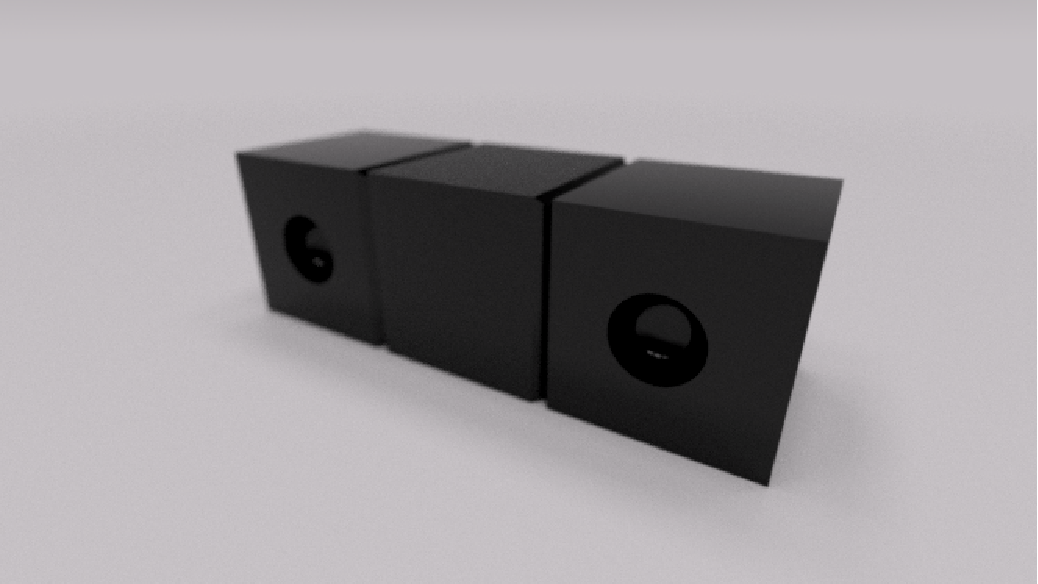
\includegraphics[width=5cm,clip]{design.pdf}
 \caption{プロジェクト内で考えたハードのデザイン}
 \label{サンプル図}
\end{minipage} &
\begin{minipage}[t]{0.5\hsize}
 \centering
 
\includegraphics[width=5cm,clip]{f.pdf}
 \caption{プロジェクト内で考えたアプリケーションのロゴ}
 \label{サンプル図}
\end{minipage}
\end{tabular}
\end{figure}

\end{center}
\section{今後の計画}
プロジェクト自体が終了しているため計画はないが今回のプロジェクトで反省点をあげる.
\begin{itemize}
\item 提出物の完成が遅くなり提出がぎりぎりになってしまった.
\item 学科が違うことでslackでのやり取りが多かったが意思疎通に齟齬などによる相違点の確認が甘く資料にミスが出た.
\item テーマ内容の詳細確認をしなかったため意見のすれ違いが起きて進捗に遅れが出た.
\end{itemize}

上記3つから事前に回避できた問題もあったためこのような機会が今後あるか定かではあるが,次からは早急に対処できるように対策を考えている.



\bibliographystyle{junsrt}
\bibliography{biblio}%「biblio.bib」というファイルが必要.

\end{document}

